This Section describes the architectures of the legacy system, based on Hudi, of IcedHops, developed during this thesis work and based on Iceberg, and the system implemented in a related thesis work \cite{manfrediReducingReadWrite2024}, based on Delta Lake. Those are the system that will be run and measured in the experimental part of this thesis work. This Section is divided into six Subsections, according to the system and the operation run over it. For each Subsection, a chart presents the operation protocol step by step.



%%%% HUDI WRITE
\subsection{Legacy system - Hudi - writing}
\label{subsec:back_sys_hudi_write}

Figure \ref{fig:hudi_write}~\footnote{For enhanced visualization, refer Figure \ref{fig:appx_hudi_write_schema}.} illustrates how data is written from the client to the offline feature store in the legacy Hopsworks system. This process is primarily divided into two synchronous phases: upload and materialization. During the upload phase, the input Pandas DataFrame is transformed into individual rows and transmitted to Kafka sequentially, one row at a time. Once the upload concludes, the client receives a notification. Meanwhile, a Spark job—Hudi Delta Streamer—operates asynchronously within the cluster from the moment the Hopsworks cluster is initialized. This job continuously fetches messages from Kafka and, upon gathering an entire table, proceeds to write the data on the table in an Apache Hudi table sitting on top of a \gls{HopsFS} system, using a columnar format. Once the materialization is completed, The Python client will receive a notification upon completion.

Similar to the pipeline, the upload and materialization phases operate asynchronously. During the experimental phase of the thesis, the materialization function was invoked to assess the overall process latency without factoring in the Hudi Delta Streamer's data retrieval interval. This approach allowed the system to trigger materialization on demand rather than waiting for the scheduled period. As a result, the experiments were able to obtain precise measurements of the total process latency.

\begin{figure}
    \begin{center}
      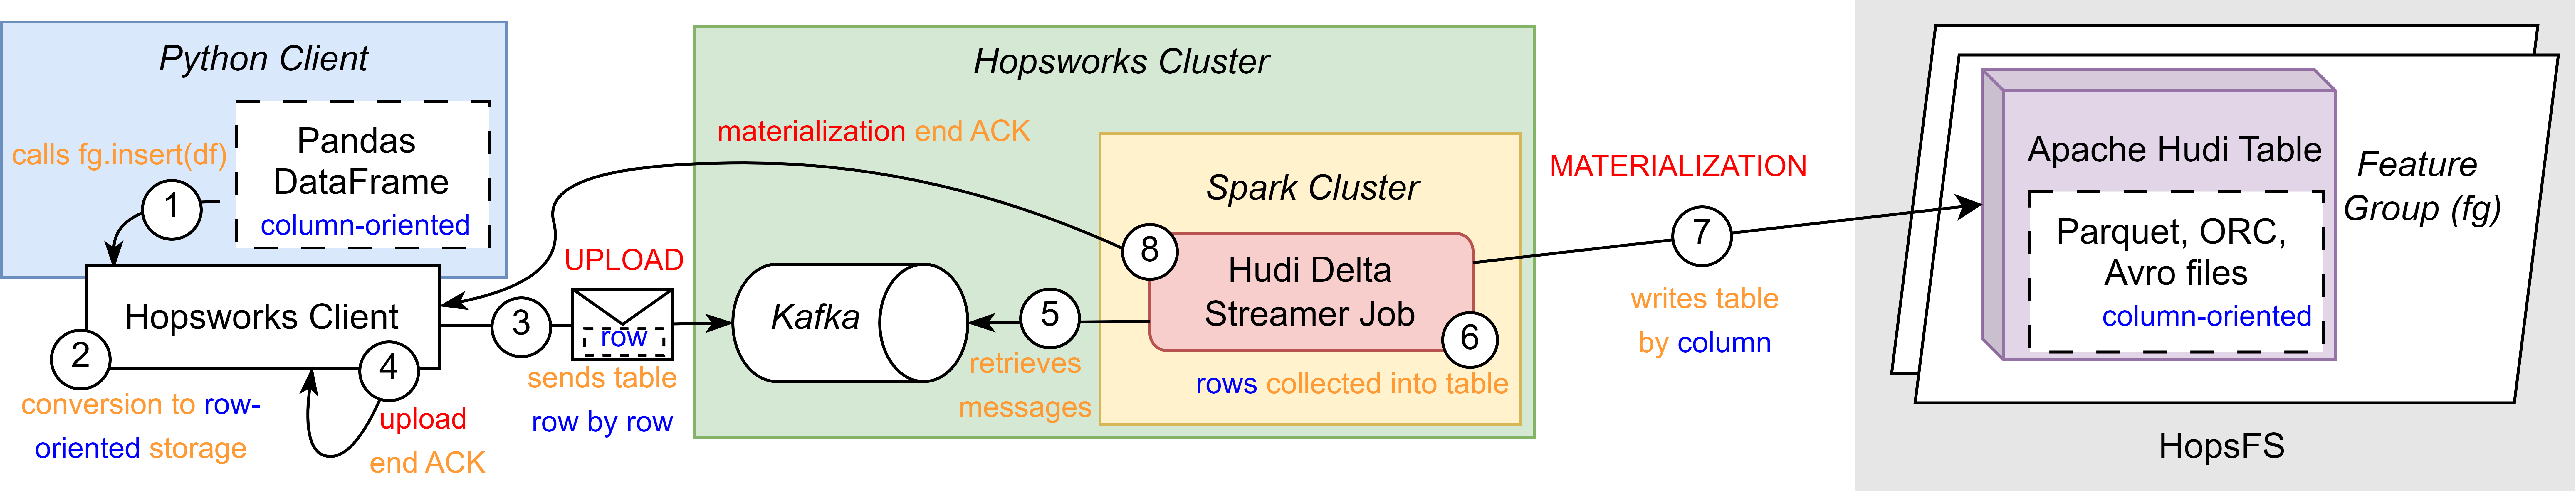
\includegraphics[width=\textwidth]{figures/2-background_and_related_work/hudi_write.png}
    \end{center}
    \caption[Legacy system - Hudi - write process]{Legacy Hudi-based system writing a DataFrame (Pandas) the Hopsworks offline feature store via a Python client.
    
    Each stage is assigned a numerical identifier. The transformation of the table format is highlighted in blue, illustrating the conversion from columns to rows and subsequently back to columns. The upload phase encompasses steps one through four, whereas the materialization phase concludes at step eight. The diagram was created based on individual interviews with Hopsworks AB developers working on the Hopsworks online and offline feature store and the related work \cite{manfrediReducingReadWrite2024} has been used as inspiration.}
    \label{fig:hudi_write}
\end{figure}



%%%% HUDI READ
\subsection{Legacy system - Hudi - reading}
\label{subsec:back_sys_hudi_read}

Figure \ref{fig:hudi_read}~\footnote{For enhanced visualization, refer Figure \ref{fig:appx_hudi_reading_schema}.}  shows the offline feature store. Conversely to the legacy system writing process, the reading process uses already a Spark alternative, which consists of a combination of an Arrow Flight server and a DuckDB instance. This was implemented by Hopsworks AI in order to direclty send the data in columnar format, without the need of convering them into row-based format.

\begin{figure}
    \begin{center}
      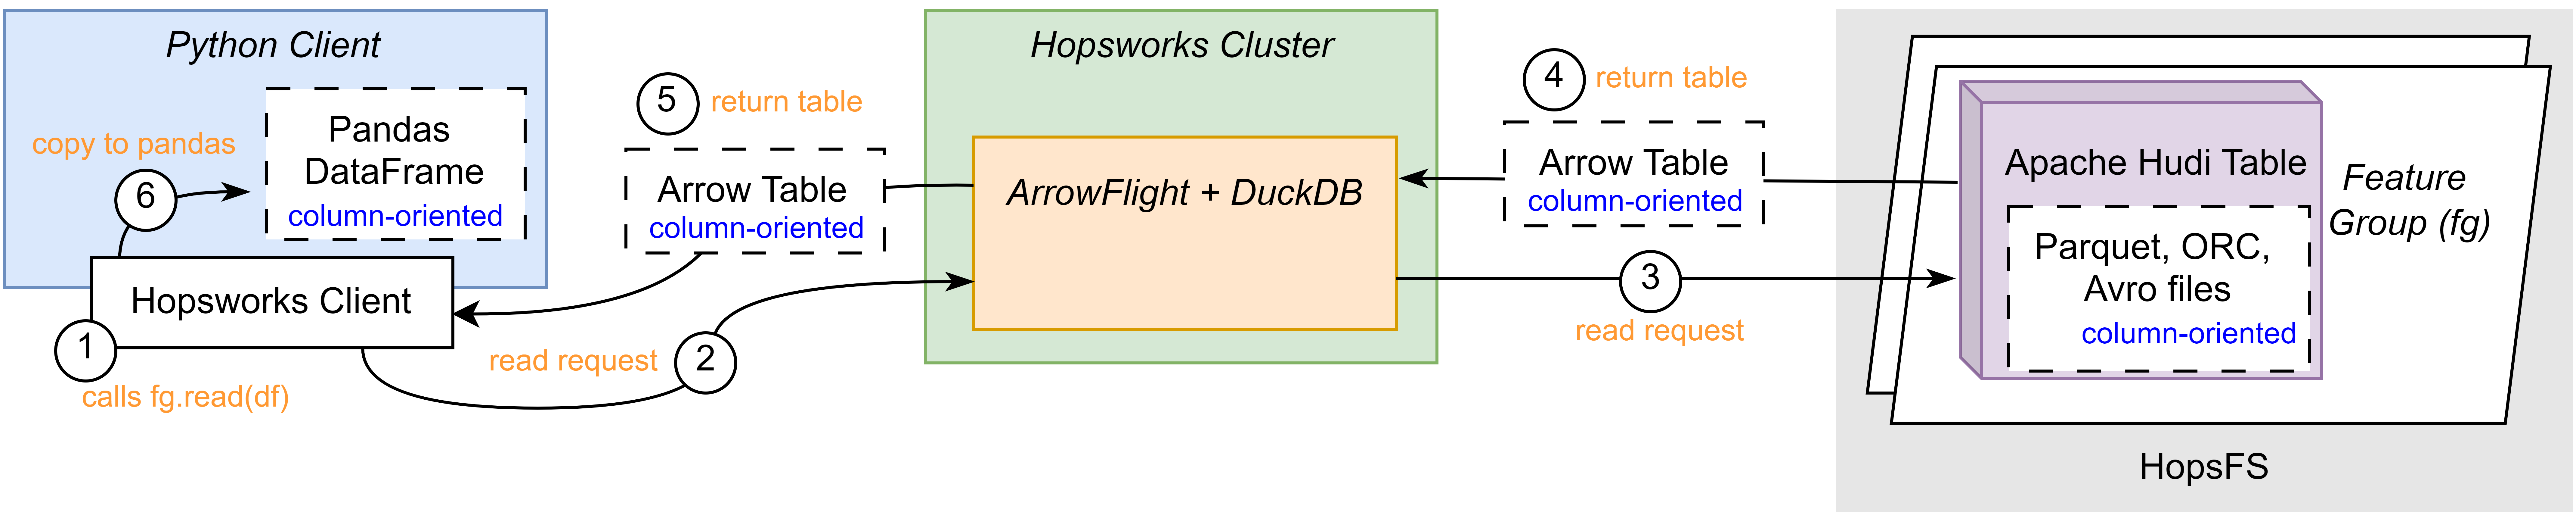
\includegraphics[width=\textwidth]{figures/2-background_and_related_work/hudi_read.png}
    \end{center}
    \caption[Legacy system - Hudi - read process]{Legacy system reading a table from the Hopsworks offline feature store and loading it into the Python client's local memory. The process is streamlined using Arrow Tables that avoid table conversion. Diagram inspired by the Hopsworks feature store paper \cite{10.1145/3626246.3653389} and by the related work \cite{manfrediReducingReadWrite2024}.}
    \label{fig:hudi_read}
\end{figure}



%%%%% ICEDHOPS WRITE
\subsection{IcedHops - writing}
\label{subsec:back_sys_iceberg_write}

Figure \ref{fig:iceberg_write} shows IcedHops writes on an Iceberg table instanced on top of \gls{HopsFS}. If first requests metadata information about the existing table to Iceberg Catalog, implemented using SQLite in the example. Once the JSON file containing the metadata is received, it reads the table location and request to read the table. IcedHops streamlines the process without passing from a server instance (Spark), removing the middle-tier from the process.

\begin{figure}
    \begin{center}
      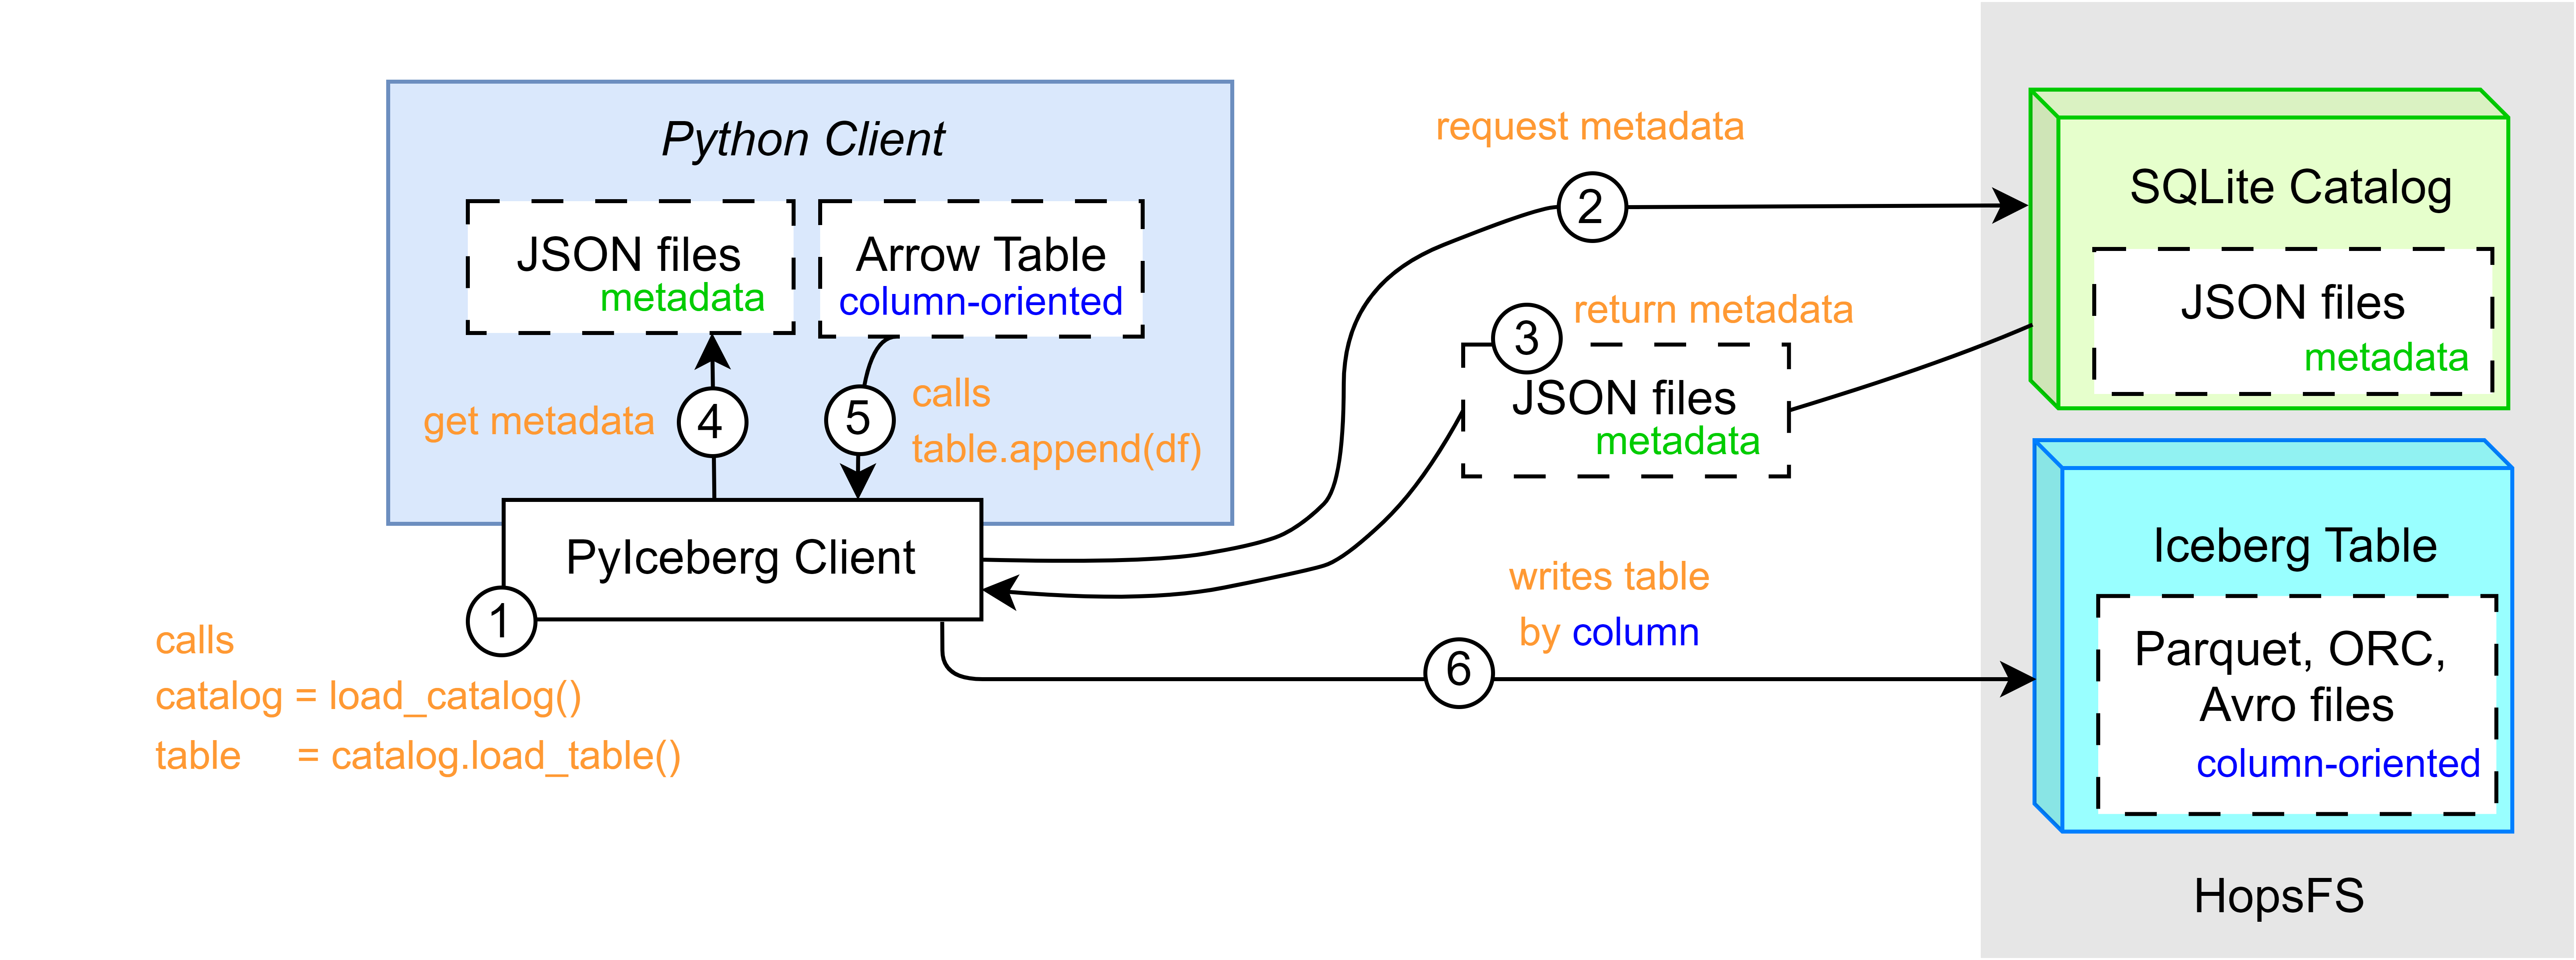
\includegraphics[width=\textwidth]{figures/2-background_and_related_work/iceberg_write.png}
    \end{center}
    \caption[IcedHops - write process]{IcedHops writing an Arrow Table from a Python client to an Iceberg Table stored on \gls{HopsFS}.}
    \label{fig:iceberg_write}
\end{figure}



%%%%% ICEDHOPS READ
\subsection{IcedHops - reading}
\label{subsec:back_sys_iceberg_read}

Figure \ref{fig:iceberg_read} shows how IcedHops reads on an Iceberg table instanced on top of \gls{HopsFS}. If first requests metadata information about the existing table to Iceberg Catalog, implemented using SQLite in the example. Once the JSON file containing the metadata is received, it reads the table location and proceed to write (append), by column, on the Iceberg Table. IcedHops streamlines the process without passing from a server instance (Arrow Flight), removing the middle-tier from the process.

\begin{figure}
    \begin{center}
      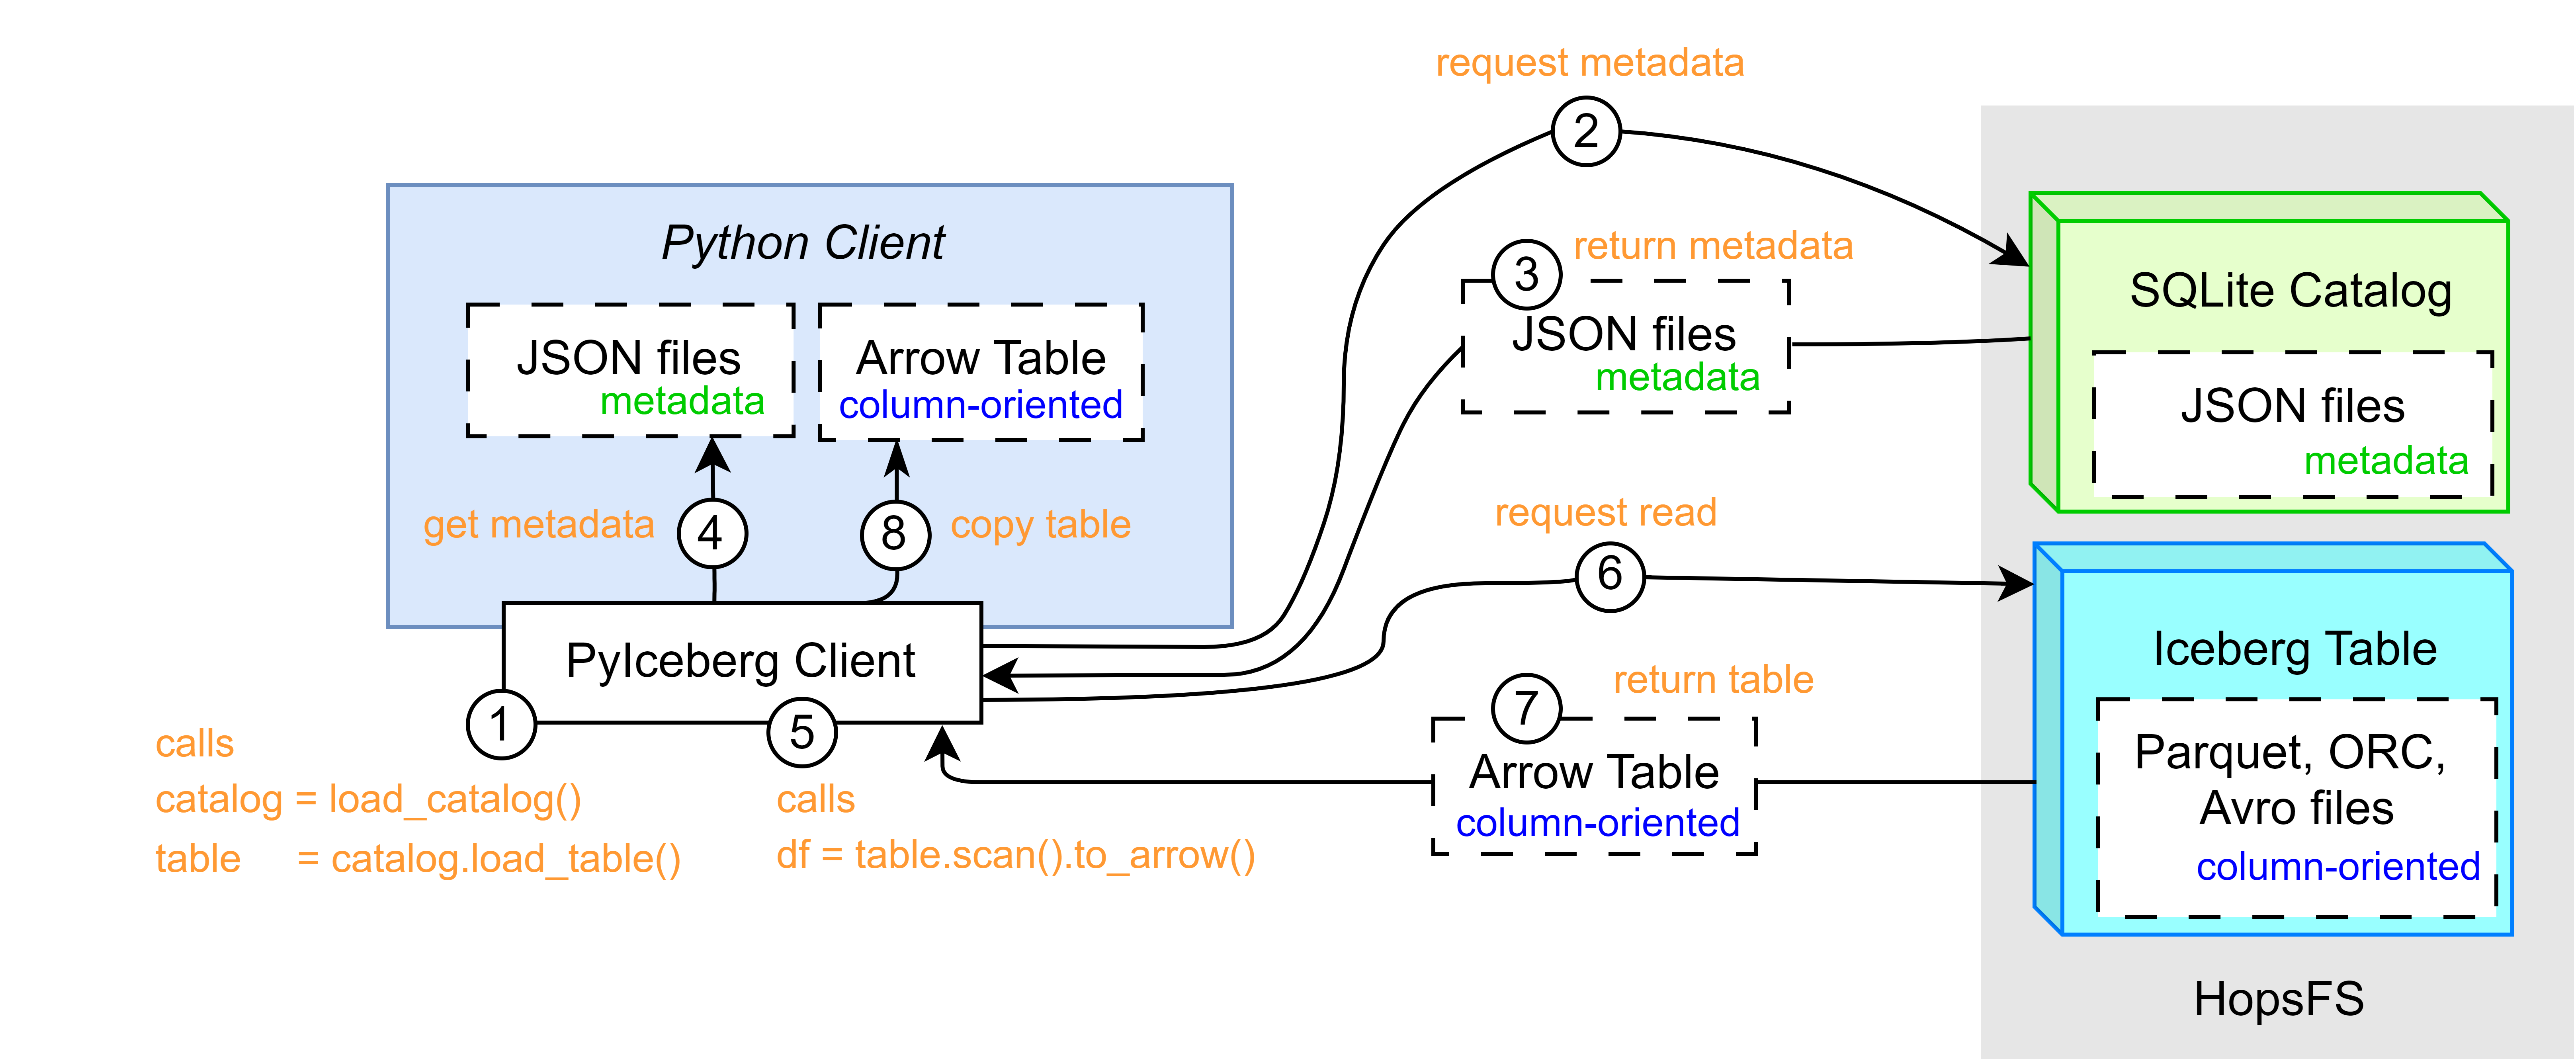
\includegraphics[width=\textwidth]{figures/2-background_and_related_work/iceberg_read.png}
    \end{center}
    \caption[IcedHops - read process]{IcedHops reading an Iceberg Table stored on \gls{HopsFS} and loading it into memory.}
    \label{fig:iceberg_read}
\end{figure}



%%%%% DELTA LAKE WRITE
\subsection{delta-rs - writing}
\label{subsec:back_sys_delta_write}

Figure \ref{fig:delta_write} shows how the delta-rs library writes on a Delta Lake table instanced on top of \gls{HopsFS}. The delta-rs library streamlines the process without passing from a server instance (Spark), removing the middle-tier from the process. In this system, the only file format supported is Parquet, while the other systems supported also ORC and Avro.

\begin{figure}
    \begin{center}
      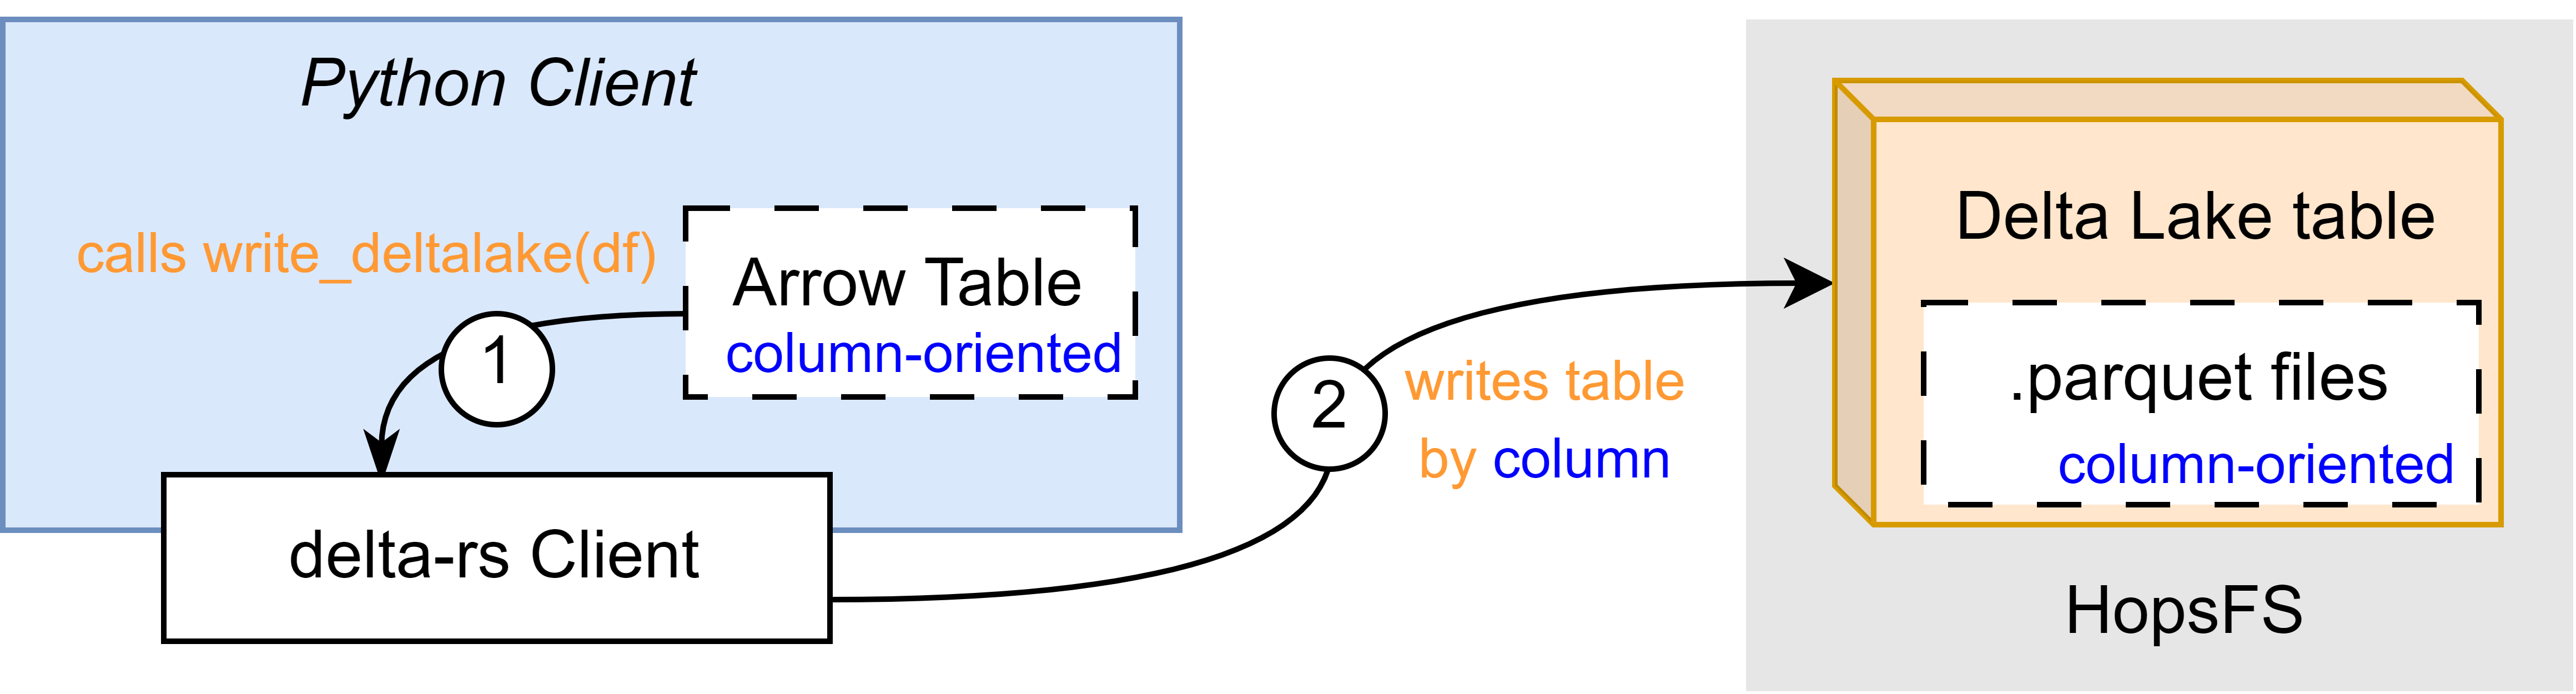
\includegraphics[width=\textwidth]{figures/2-background_and_related_work/delta_write.png}
    \end{center}
    \caption[delta-rs - write process]{Delta-rs library writing an Arrow Table from a Python client to a Delta Lake table stored on \gls{HopsFS}. Diagram inspired by the related work \cite{manfrediReducingReadWrite2024}.}
    \label{fig:delta_write}
\end{figure}



%%%%% DELTA LAKE READ
\subsection{delta-rs - reading}
\label{subsec:back_sys_delta_read}

Figure \ref{fig:delta_read} shows how the delta-rs library reads a Delta Lake table instanced on top of \gls{HopsFS}. The delta-rs library streamlines the process without passing from a server instance (Arrow Flight), removing the middle-tier from the process. In this system, the only file format supported is Parquet, while the other systems supported also ORC and Avro.

\begin{figure}
    \begin{center}
      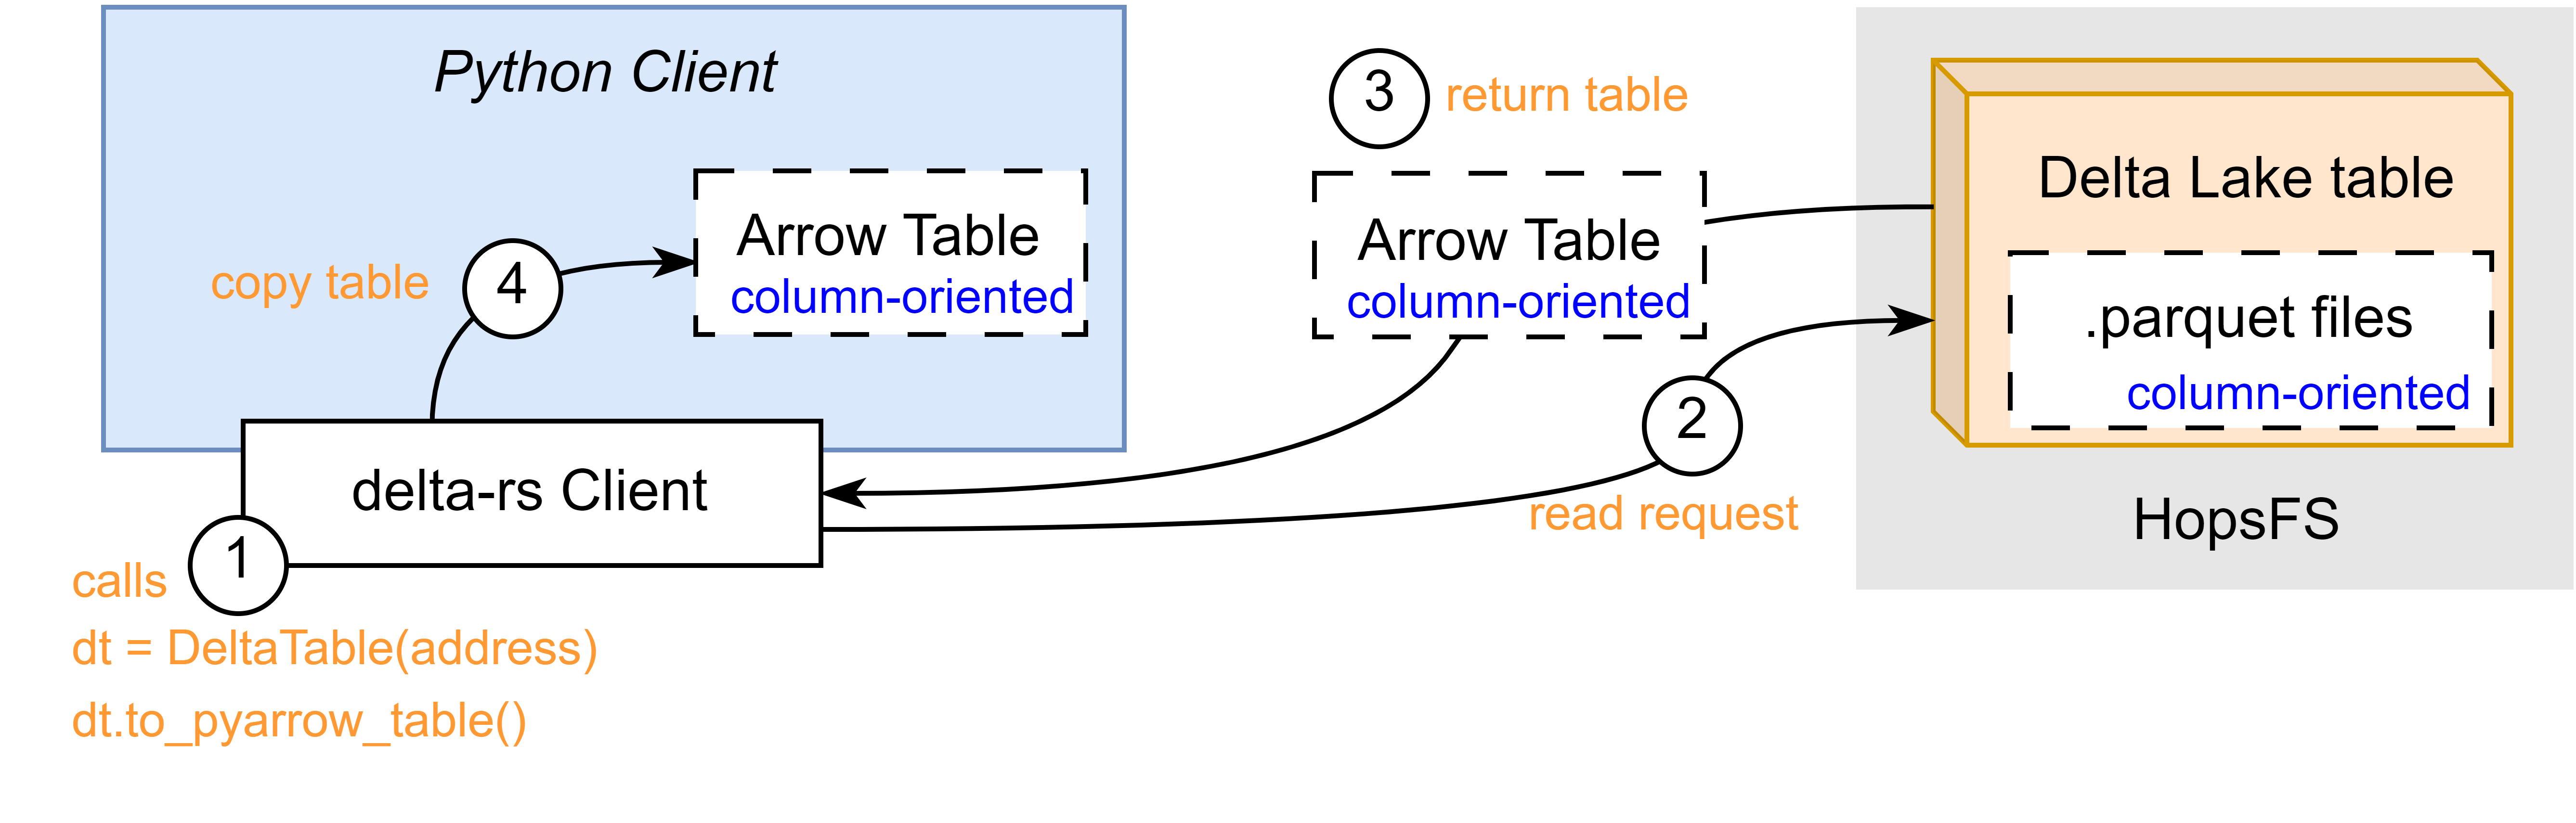
\includegraphics[width=\textwidth]{figures/2-background_and_related_work/delta_read.png}
    \end{center}
    \caption[delta-rs - read process]{Delta-rs library reading a Delta Lake table stored in \gls{HopsFS} and loading it into memory. Diagram inspired by the related work \cite{manfrediReducingReadWrite2024}.}
    \label{fig:delta_read}
\end{figure}